\documentclass[14pts]{beamer}
\usetheme{metropolis}           % Use metropolis theme
\usepackage{graphicx}
\usepackage{tikz}
\usetikzlibrary{automata, positioning}
\usepackage{amsmath, amssymb, amsfonts, amsthm}
\usepackage{bm}            % For bold maths \bm{...}
% \usepackage{ wasysym }    % for \smiley
% \usepackage{mathdots}   % for different ellipses
% \usepackage{multirow}   % for merging multiple rows
\usepackage{hyperref}   % for links
% \usepackage[linguistics]{forest} % for drawing trees
% \usepackage{fancyvrb}   % for code insertion
% \usepackage{float}        % for forcing figure position \begin{figure}[H]
% \usepackage{xcolor}        % for colors
% \usepackage{tcolorbox}    % for colorful boxes
% \usepackage{comment}     % for multiline comments
% \usepackage{enumitem}    % for changing labeling of a ordered list. Very powerful [label = {  (\alph*).  }] for (a). (b). etc.

\setbeamercolor{block body}{bg=mDarkTeal!30}
\setbeamercolor{block title}{bg=mDarkTeal,fg=black!2}
\setbeamercovered{transparent}

\title{Büchi Automata}
\date{\today}
\author{Vansh, Pinakin, Aayush, Bhanu}
\institute{Indian Institute of Science, Bangalore}


\begin{document}
  \maketitle
  \tableofcontents  
  \section{Regular Expressions and $\omega$-Regular Expressions}
  \begin{frame}{Regular Expressions over $\Sigma$}
    \begin{block}{Definition}
      A regular expression is a sequence of characters that define a search pattern.
      \[\alpha := \phi \mid A \mid \alpha_1 + \alpha_2 \mid \alpha_1\cdot\alpha_2 \mid \alpha^*\]
      Where $A$ is an alphabet and $\phi$ is the empty string.
    \end{block}
    Some semantics used throughout the presentation:
    \begin{itemize}
      \item<1-> $\alpha_1 + \alpha_2$ is the union of $\alpha_1$ and $\alpha_2$
      \item<2-> $\alpha_1\cdot\alpha_2$ is the concatenation of $\alpha_1$ and $\alpha_2$
      \item<3-> $\alpha^*$ is the Kleene closure of $\alpha$
      \item<4-> $\mathcal{L}(\phi) = \phi$, $\mathcal{L}(A) = \{A\}$ and $\mathcal{L}(\epsilon)= \{\epsilon\}$
    \end{itemize}
  \end{frame}
  \begin{frame}{$\omega$-Regular Expression}
    \begin{definition}
      $\omega$-regular expression = regex + $\omega$-operator $\alpha^\omega$\\
      Where we choose any string generated by $\alpha$ and repeat it infinitely many times, denoted by $\omega$-operator.
      \[\text{for} \hspace{1mm} \mathcal{L} \subseteq \Sigma^*:\]
      \[\mathcal{L}^{\omega} = \{w_1w_2w_3\cdots: w_i \in \mathcal{L}\hspace{1mm} \forall i \geq 1\} \]
    \end{definition}
    \onslide<2->{$$\mathcal{L}(\omega) \subseteq \Sigma^{\omega} \text{ if } \epsilon \notin \mathcal{L}$$}
    \onslide<3->{\begin{itemize}
        \item Kleene Star: 'finite repetition'
        \item $\omega$-operator: 'infinite repetition'
    \end{itemize}}
  \end{frame}

  {\setbeamercovered{invisible}
    \begin{frame}{Syntax and semantics of $\omega$-regular expressions}
      \begin{definition}
        Syntax of $\omega$-regular expressions over alphabet $\Sigma$:
        \[\gamma  =  \alpha_1\cdot\beta_1^{\omega}+ \cdots + \alpha_n\cdot\beta_n^{\omega} \]
        $\alpha_i, \beta_i$ are regular expressions over $\Sigma$ such that $\epsilon \notin \mathcal{L}(\beta_i)$
      \end{definition}
      \onslide<2->{The language generated by $\gamma$ is: 
        \[\mathcal{L}_{\omega}(\gamma) = \bigcup_{1 \leq i \leq n}\mathcal{L}(\alpha_i)\mathcal{L}(\beta_i)^{\omega} \subseteq \Sigma^{\omega}\]}
      \onslide<3->{\begin{example}
          The language of $(A^*B)^{\omega} = $ set of all infinite words containing  infinitely many $B$'s
        \end{example}}
    \end{frame}
    \begin{frame}{$\omega$ Regular Language}
      \begin{block}{$\omega$ Regular Language}
        A language $\mathcal{L} \subseteq \Sigma^{\omega}$ is called $\omega$-regular iff there exists an $\omega$ regular expression
        such that $\mathcal{L} = \mathcal{L}_{\omega}(\gamma)$
      \end{block}
    \end{frame}}
  \begin{frame}{$\omega$ - regex example}
    \begin{itemize}
      \item<1> Alphabet $\Sigma = \{a, b\}$ such that the set of all infinite words contain finitely
      many $a$'s.
      \[(a + b)^*b^{\omega}\]
      \item<2> Set of all infinite words where each $a$ is followed immediately by letter $b$.
      \[(b^*.a.b)^*.b^{\omega} + (b^*.a.b)^{\omega}\]
    \end{itemize}
  \end{frame}
  \section{Non-Deterministic Büchi Automata}
  \begin{frame}{Büchi Automata (NBA)}
    A Büchi automaton is a method of defining a set of $\omega$ words over a finite alphabet $\Sigma$
    \begin{definition}
      A (non-deterministic) Büchi automaton is a tuple $A = (Q, \Sigma, \delta, Q_0, F)$ where:
      \begin{itemize}
        \item Q is a finite set of states
        \item $\Sigma$ is a finite alphabet
        \item $Q_0 \subseteq Q$ set of initial states
        \item $\delta \subseteq  Q \times \Sigma \times Q$ is the transition relation.
        \item $F$ is the set of final states.
      \end{itemize}
    \end{definition}
    % A $\omega$-word is accepted by a Buchi automaton if it is spelt out by an infinite path
    % which, starting from the initial node, visits some final state infinitely often. 
  \end{frame}
  \begin{frame}{Büchi Automata (NBA)}
    \begin{block}{Acceptance}
    Let $A_0A_1A_2\cdots\in\Sigma^{\omega}$ be a run of a word, and $\pi$ be the sequence of 
    states visited:
    \[\pi = q_0q_1q_2\cdots \text{ where } q_0 \in Q_0\]
    \[q_{i+1} \in \delta(q_i, A_i) \text{ for } i \geq 0\]
    We say that  run $\pi$ is accepted if there exist infinitely many $i$'s such that $q_i \in F$.
    \end{block}
    \onslide<2->{The language recognised by A, written $\mathcal{L}(A)$, is the set of 
    $\omega$-words accepted by A. \\}
  \end{frame}
  {\setbeamercovered{invisible}
    \begin{frame}{NBA Example}
    \begin{columns}[T]
      \column<1->{0.5\textwidth}
      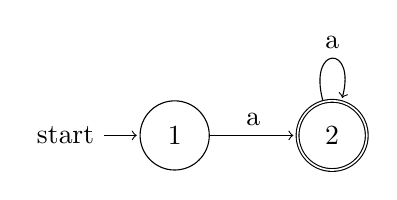
\begin{tikzpicture}[shorten >=1pt,node distance=2cm,on grid,auto] 
        \node[state,initial] (q_0)   {$1$}; 
        \node[state,accepting] (q_1) [right=of q_0] {$2$}; 
        \path[->] 
        (q_0) edge  node {a} (q_1)
        (q_1) edge [loop above] node {a} ();
        ; 
      \end{tikzpicture}

      \onslide<2->{This automaton accepts the language of all $\omega$-words over $\{a\}$ that contain infinitely many $a$'s.
      \[\mathcal{L}_{\omega}(A_1) = \{a\}^{\omega}\]}
      \column<3->{0.5\textwidth}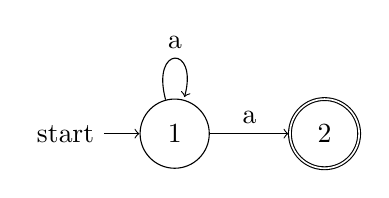
\begin{tikzpicture} 
        \node[state,initial] (q_0)   {$1$}; 
        \node[state, accepting] (q_1) [right=of q_0] {$2$}; 
        \path[->] 
        (q_0) edge [above] node {a} (q_1)
        (q_0) edge [loop above] node {a} ();
        ; 
      \end{tikzpicture}

      \onslide<4->{This automaton does not accept any $\omega$-words.
      \[\mathcal{L}_{\omega}(A_2) = \phi\]}
    \end{columns} \vspace*{0.3in}
    \onslide<5>{In NBA "perspective", both languages are different. }
  \end{frame}}
  {\setbeamercovered{invisible}
    \begin{frame}{NBA Example (Language accepted by NFA)}
    \begin{columns}[T]
      \column<1->{0.5\textwidth}
      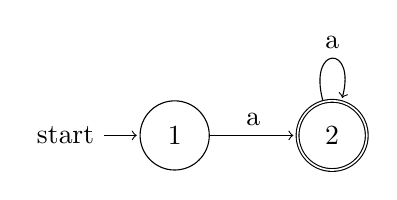
\begin{tikzpicture}[shorten >=1pt,node distance=2cm,on grid,auto] 
        \node[state,initial] (q_0)   {$1$}; 
        \node[state,accepting] (q_1) [right=of q_0] {$2$}; 
        \path[->] 
        (q_0) edge  node {a} (q_1)
        (q_1) edge [loop above] node {a} ();
        ; 
      \end{tikzpicture}

      The language accepted by the automaton $A_1$, $\mathcal{L}(A_1) = \{a^{n+1} \mid n \in N\}$
      
      \column<2->{0.5\textwidth}
      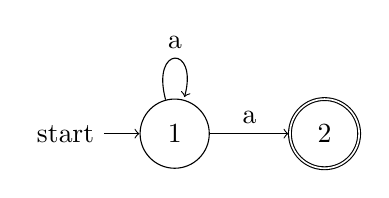
\begin{tikzpicture} \node[state,initial] (q_0)   {$1$}; 
        \node[state, accepting] (q_1) [right=of q_0] {$2$}; 
        \path[->] 
        (q_0) edge [above] node {a} (q_1)
        (q_0) edge [loop above] node {a} ();
        ; 
      \end{tikzpicture}

      The language accepted by the automaton $A_2$, $\mathcal{L}(A_2) = \{a^{n+1} \mid n \in N\}$
    \end{columns}
    \vspace*{0.4in}
    \onslide<3->{We can see that, the languages accepted by the automata $A_1$ and $A_2$ are same in NFA "perspective".\\
    Thus both automaton are equivalent in NFA "perspective", but different in NBA "perspective".}
  \end{frame}}
  \begin{frame}{Example of NBA over $\Sigma = \{a, b\}$}
    \begin{columns}
      \column{0.5\textwidth}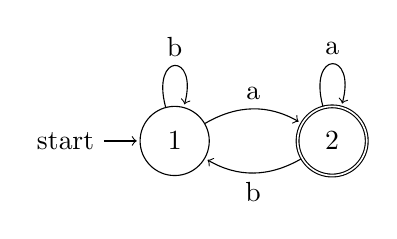
\begin{tikzpicture}[shorten >=1pt,node distance=2cm,on grid,auto] 
        \node[state,initial] (q_0)   {$1$}; 
        \node[state,accepting] (q_1) [right=of q_0] {$2$}; 
        \path[->] 
        (q_0) edge[bend left]  node {a} (q_1)
        (q_1) edge[bend left] node {b} (q_0)
        (q_1) edge [loop above] node {a} ()
        (q_0) edge [loop above] node {b} ();
        ; 
      \end{tikzpicture}
      \column<2->{0.5\textwidth} Accepted language: \\ Set of all infinite words that contain infinitely many a's \\
      $\mathcal{L}(M) = (a^*b)^{\omega}$
    \end{columns}
  \end{frame}
  \section{Characterizing Büchi Recognisable Languages}
    \begin{frame}{Converting NBA to $\omega$-regular expression}
      \begin{theorem}
        A language is Buchi recognisable iff it is $\omega$ regular.
      \end{theorem}
      \onslide<2->{\begin{proof}
      $(\implies )$ Converting NBA to $\omega$ regular language.\\
      Let $A$ be an NBA $(Q, \Sigma, \delta, Q_0, F)$ and $q, p \in Q$.\\
      Let $A_{q, p}$ be the NFA $(Q, \Sigma, \delta, q, \{p\}).$ Then:\\
                                \[\mathcal{L}{\omega}(A) = \bigcup_{q\in Q_0}\bigcup_{p \in F}\mathcal{L}(A_{q, p})(\mathcal{L}(A_{p, p}) \backslash \{\epsilon\})^{\omega}\]  
    is $\omega$ regular  as $\mathcal{L}(A_{q, p})$ and $\mathcal{L}(A_{p, p}) \backslash \{\epsilon\}$  are regular by definition.  
      \end{proof}}
    \end{frame}
    \begin{frame}{Converting NBA to $\omega$-regular expression}
      \begin{figure}
        \centering
        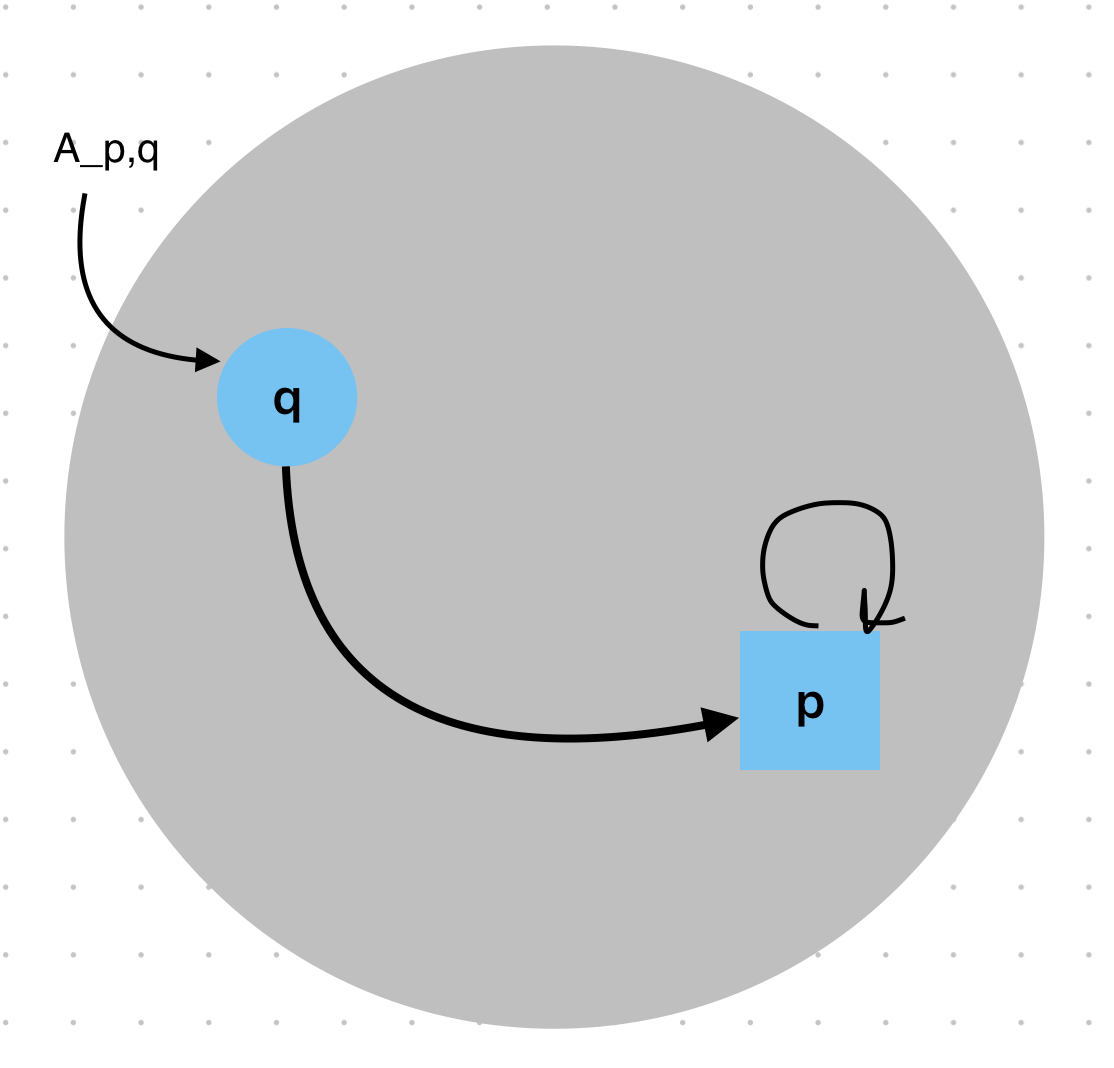
\includegraphics[width=0.8\textwidth]{photo1.png}
        \caption{NBA for $\mathcal{L}(A) = (a^*b)^{\omega}$}
      \end{figure}
    \end{frame}
    {\setbeamercovered{invisible}
      \begin{frame}{Example: Converting NBA to $\omega$-regular expression}
      \only<1>{\begin{figure}
        \centering
        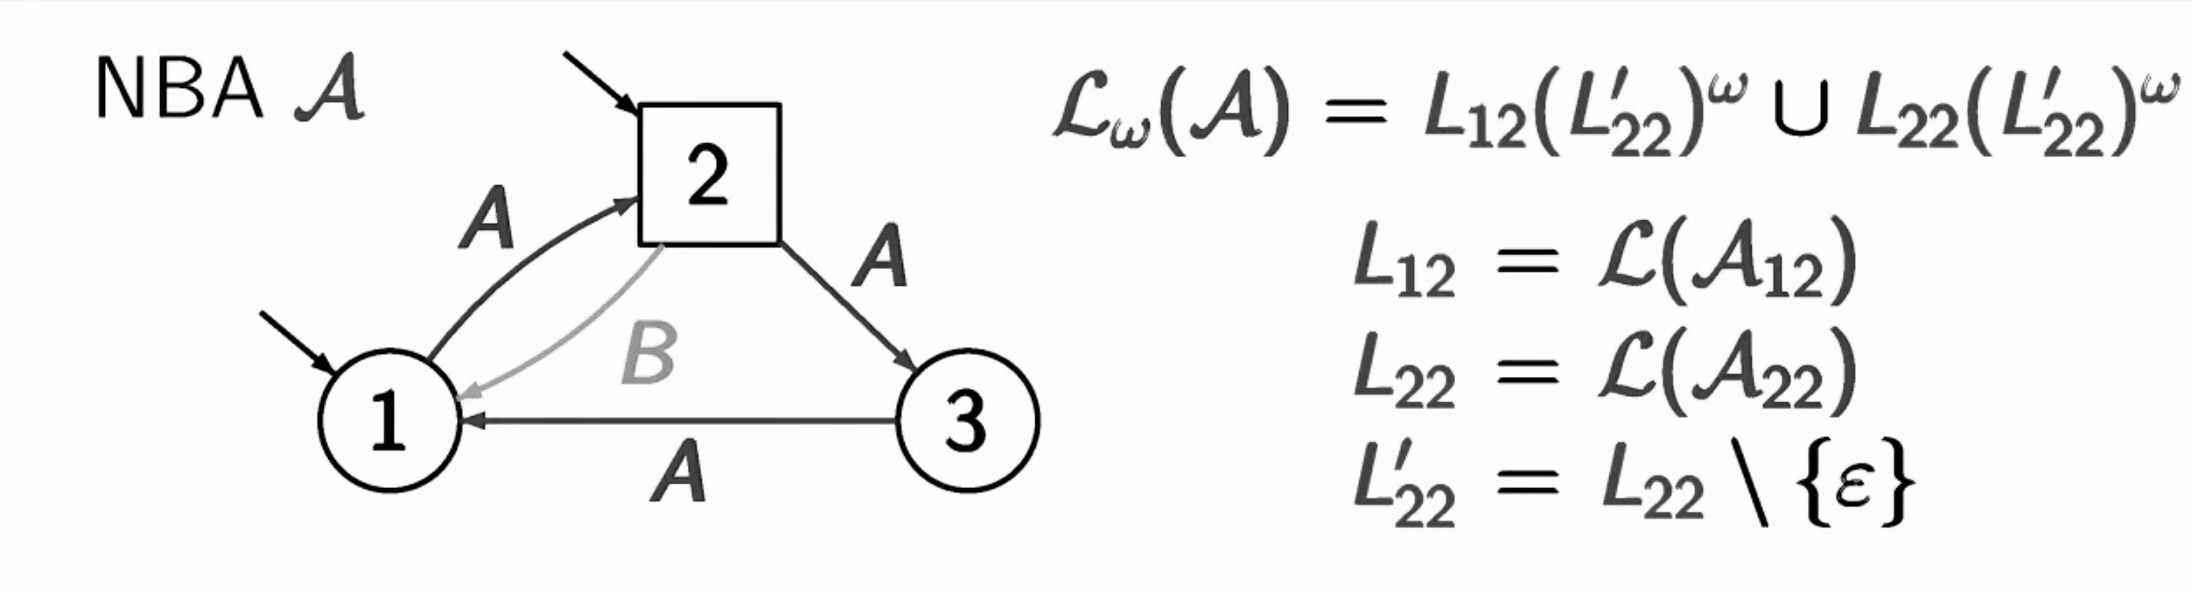
\includegraphics[width=0.8\textwidth]{photo7-1.jpeg}
      \end{figure}}
      \only<2>{\begin{figure}
        \centering
        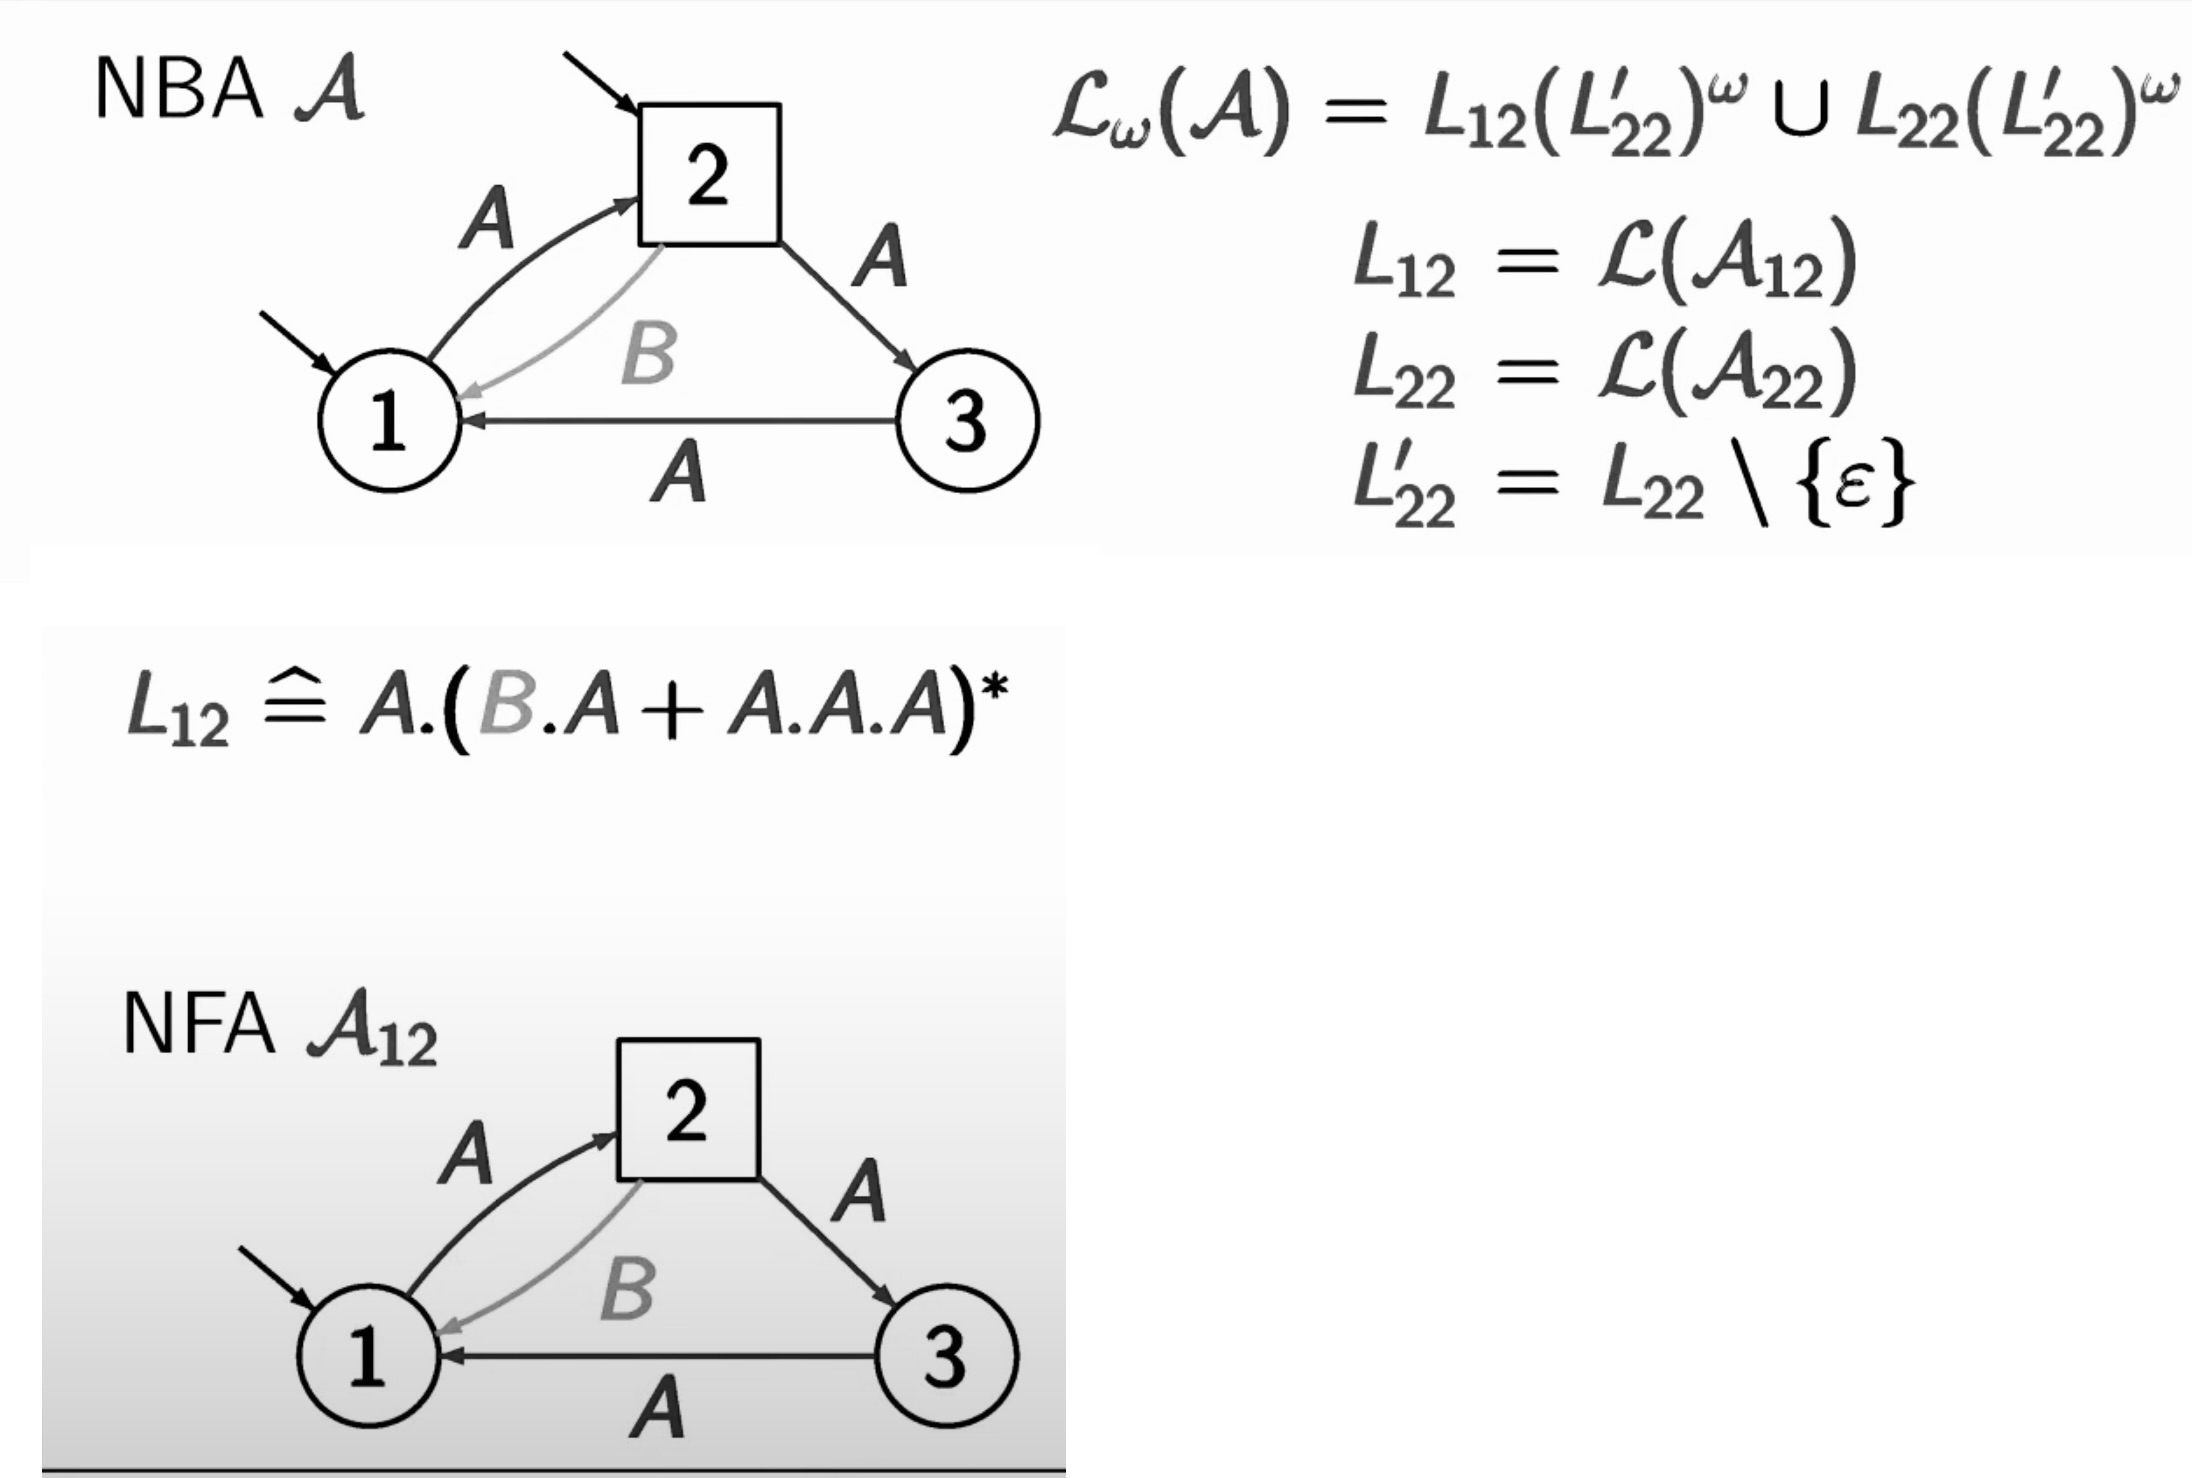
\includegraphics[width=0.8\textwidth]{photo7-2.jpeg}
      \end{figure}}
      \only<3>{\begin{figure}
        \centering
        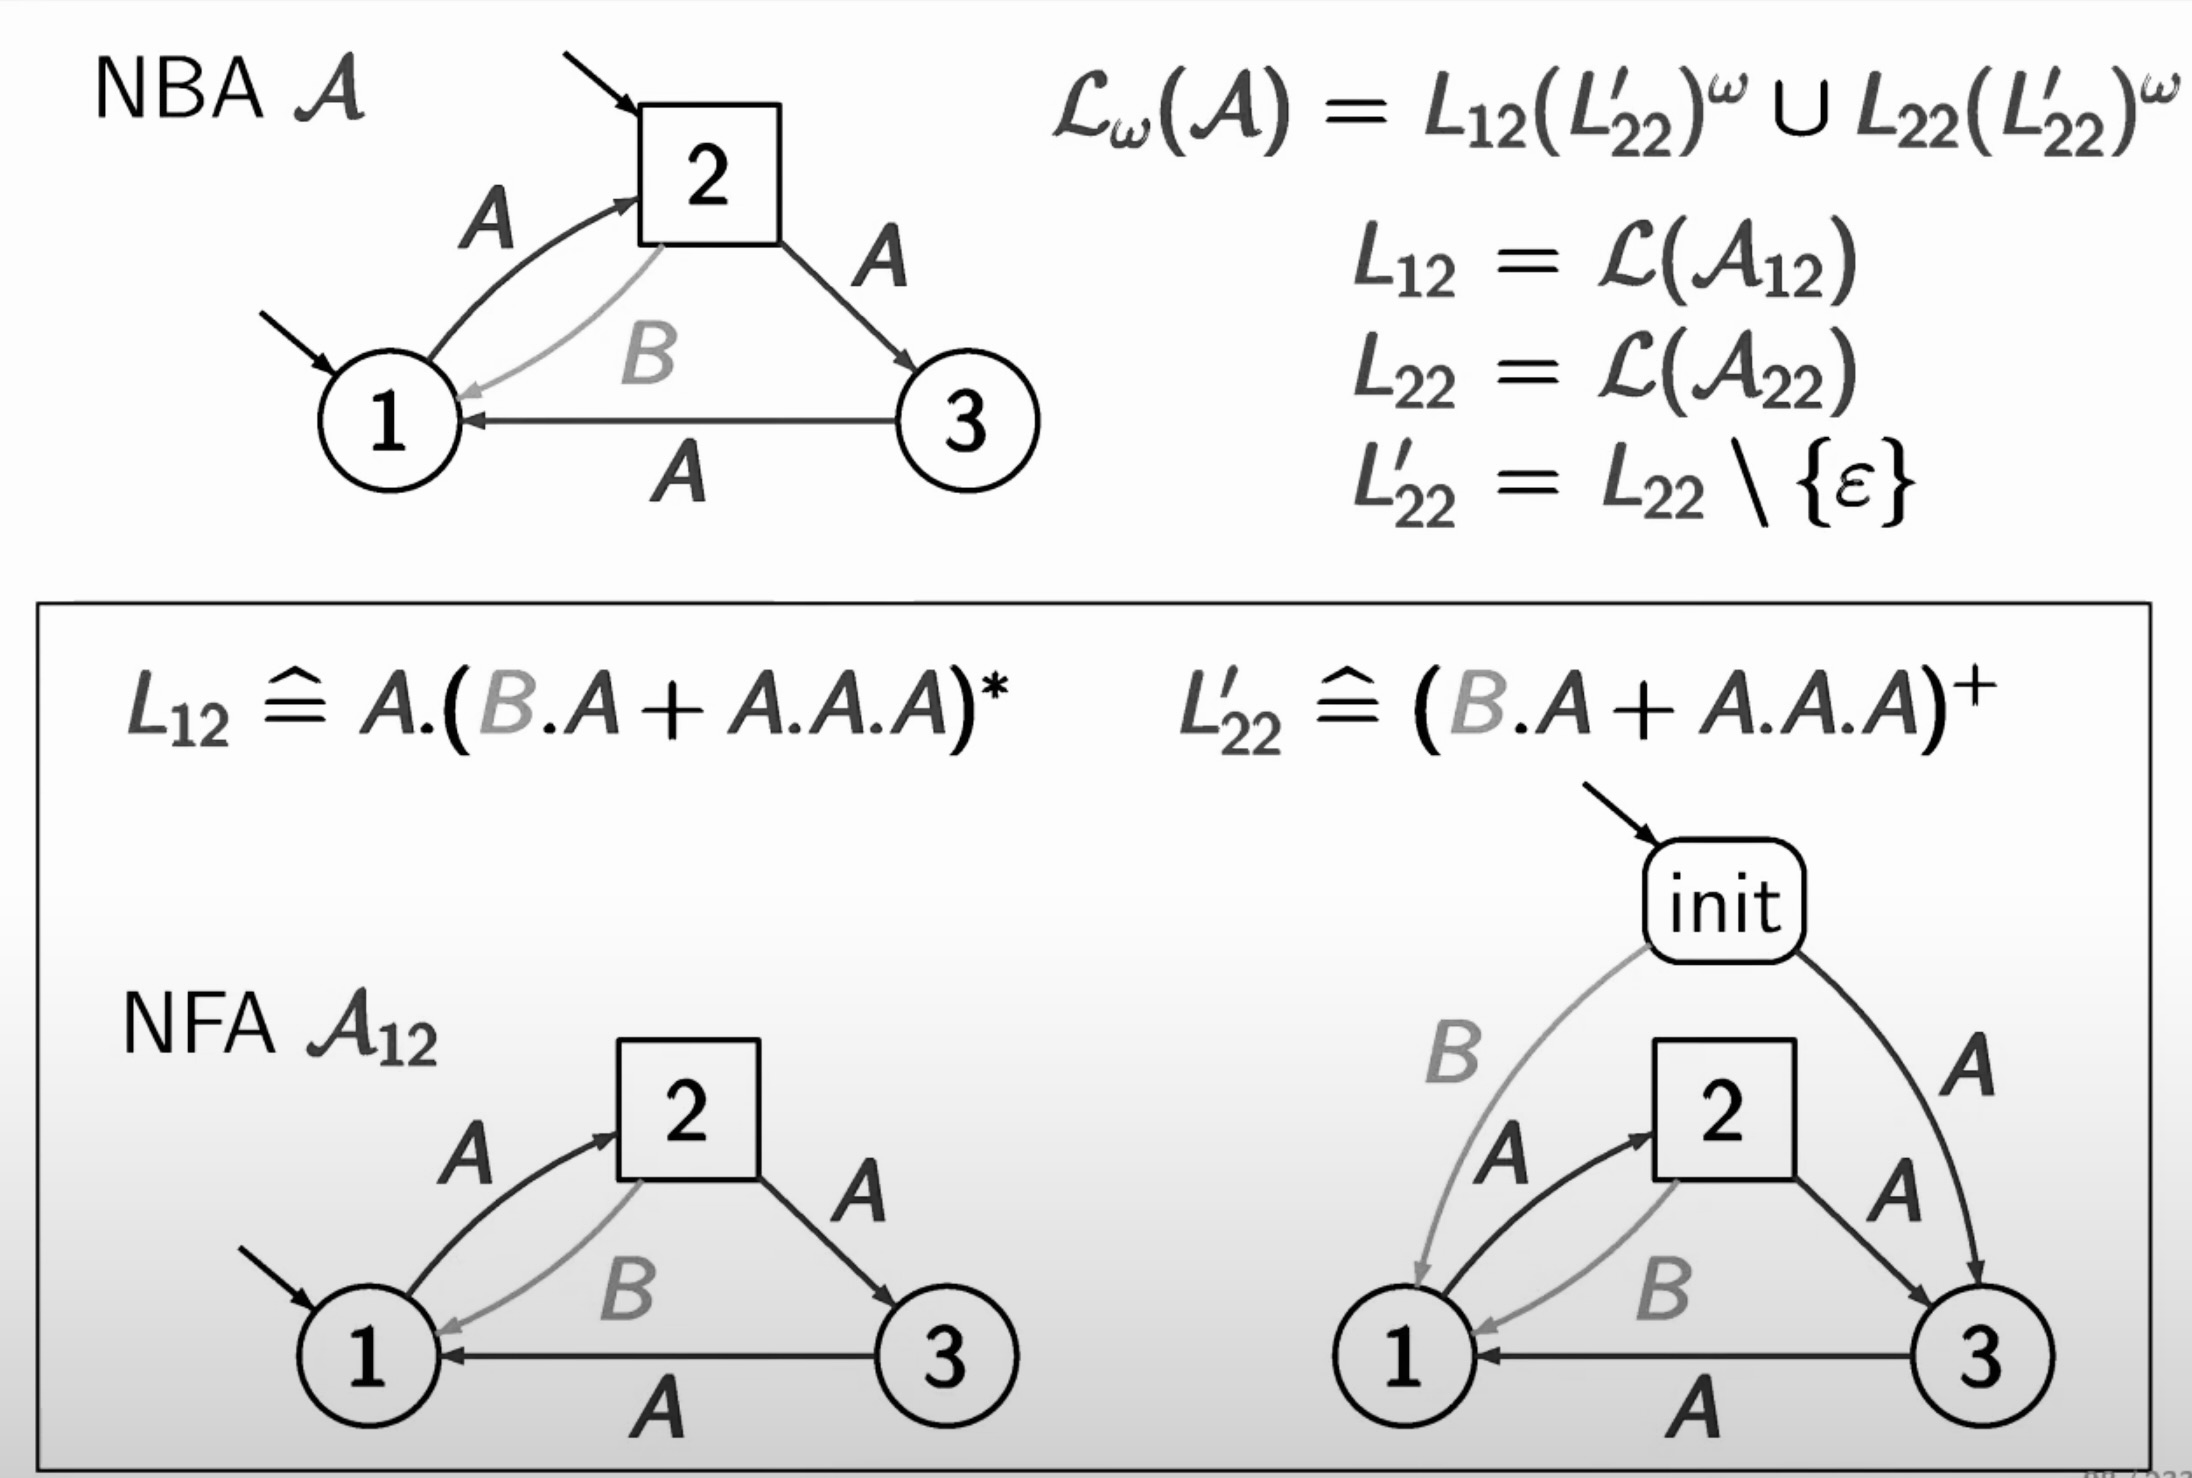
\includegraphics[width=0.8\textwidth]{photo7-3.jpeg}
      \end{figure}}
    \end{frame}}
    \begin{frame}{From $\omega$-regular expression to NBA}
      \begin{proof}
      $(\impliedby)$ Converting $\omega$ regular expression to NBA.\\
      Let $\gamma$ be an $\omega$ regular expression over $\Sigma$.\\
      \[\gamma = \alpha_1\cdot\beta_1^{\omega} + \cdots + \alpha_n\cdot\beta_n^{\omega}\]
      there exists an NBA A, with $\mathcal{L}{\omega}(A) = \mathcal{L}{\omega}(\gamma)$\\
      \textbf<overlay specification>{Proof:} consider NFA $\mathcal{A}_i$ for $\alpha_i$ and $\mathcal{B}_i$ for $\beta_i$\\
        \begin{itemize}
            \item construct NBA $\mathcal{B}_i^{\omega} $ for $\beta_i^{\omega}$
            \item construct NBA $\mathcal{C}_i = \mathcal{A}_i\cdot\mathcal{B}_i^{\omega}$ for $\alpha_i\cdot\beta_i^{\omega}$
            \item construct NBA for $\bigcup_{1\leq i \leq n}\mathcal{L}_{\omega}(\mathcal{C}_i)$
        \end{itemize}
        \end{proof}
        We proceed the proof by showing that the set of Buchi recognisable languages satisy the following closure properties:
    \end{frame}
    \begin{frame}{Closure under Finite Union}
        \begin{block}{Finite Union}
            Let $A_1$ = $(Q_1, \Sigma, \delta_1, Q_{01}, F_1)$ and $A_2$ = $(Q_2, \Sigma, \delta_2, Q_{02}, F_2)$ be two NBA's. Then the language $\mathcal{L}(A_1) \cup \mathcal{L}(A_2)$ is Buchi recognisable.
        \end{block}
        \onslide<2->{\begin{block}{Proof.}
          Just take the union of the two automata !
        \end{block}}
    \end{frame}
    \begin{frame}{Concatenation of NFA and NBA }
    \begin{block}{Concatenation}  
      If $L(A_1)$ is regular and $L_{\omega}(A_2)$ is Buchi recognisable then $L(A_1)L_{\omega}(A_2)$ is Buchi recognisable.
    \end{block}
    \end{frame}
    \begin{frame}{Concatenation of NFA and NBA}
      \begin{figure}
        \centering
        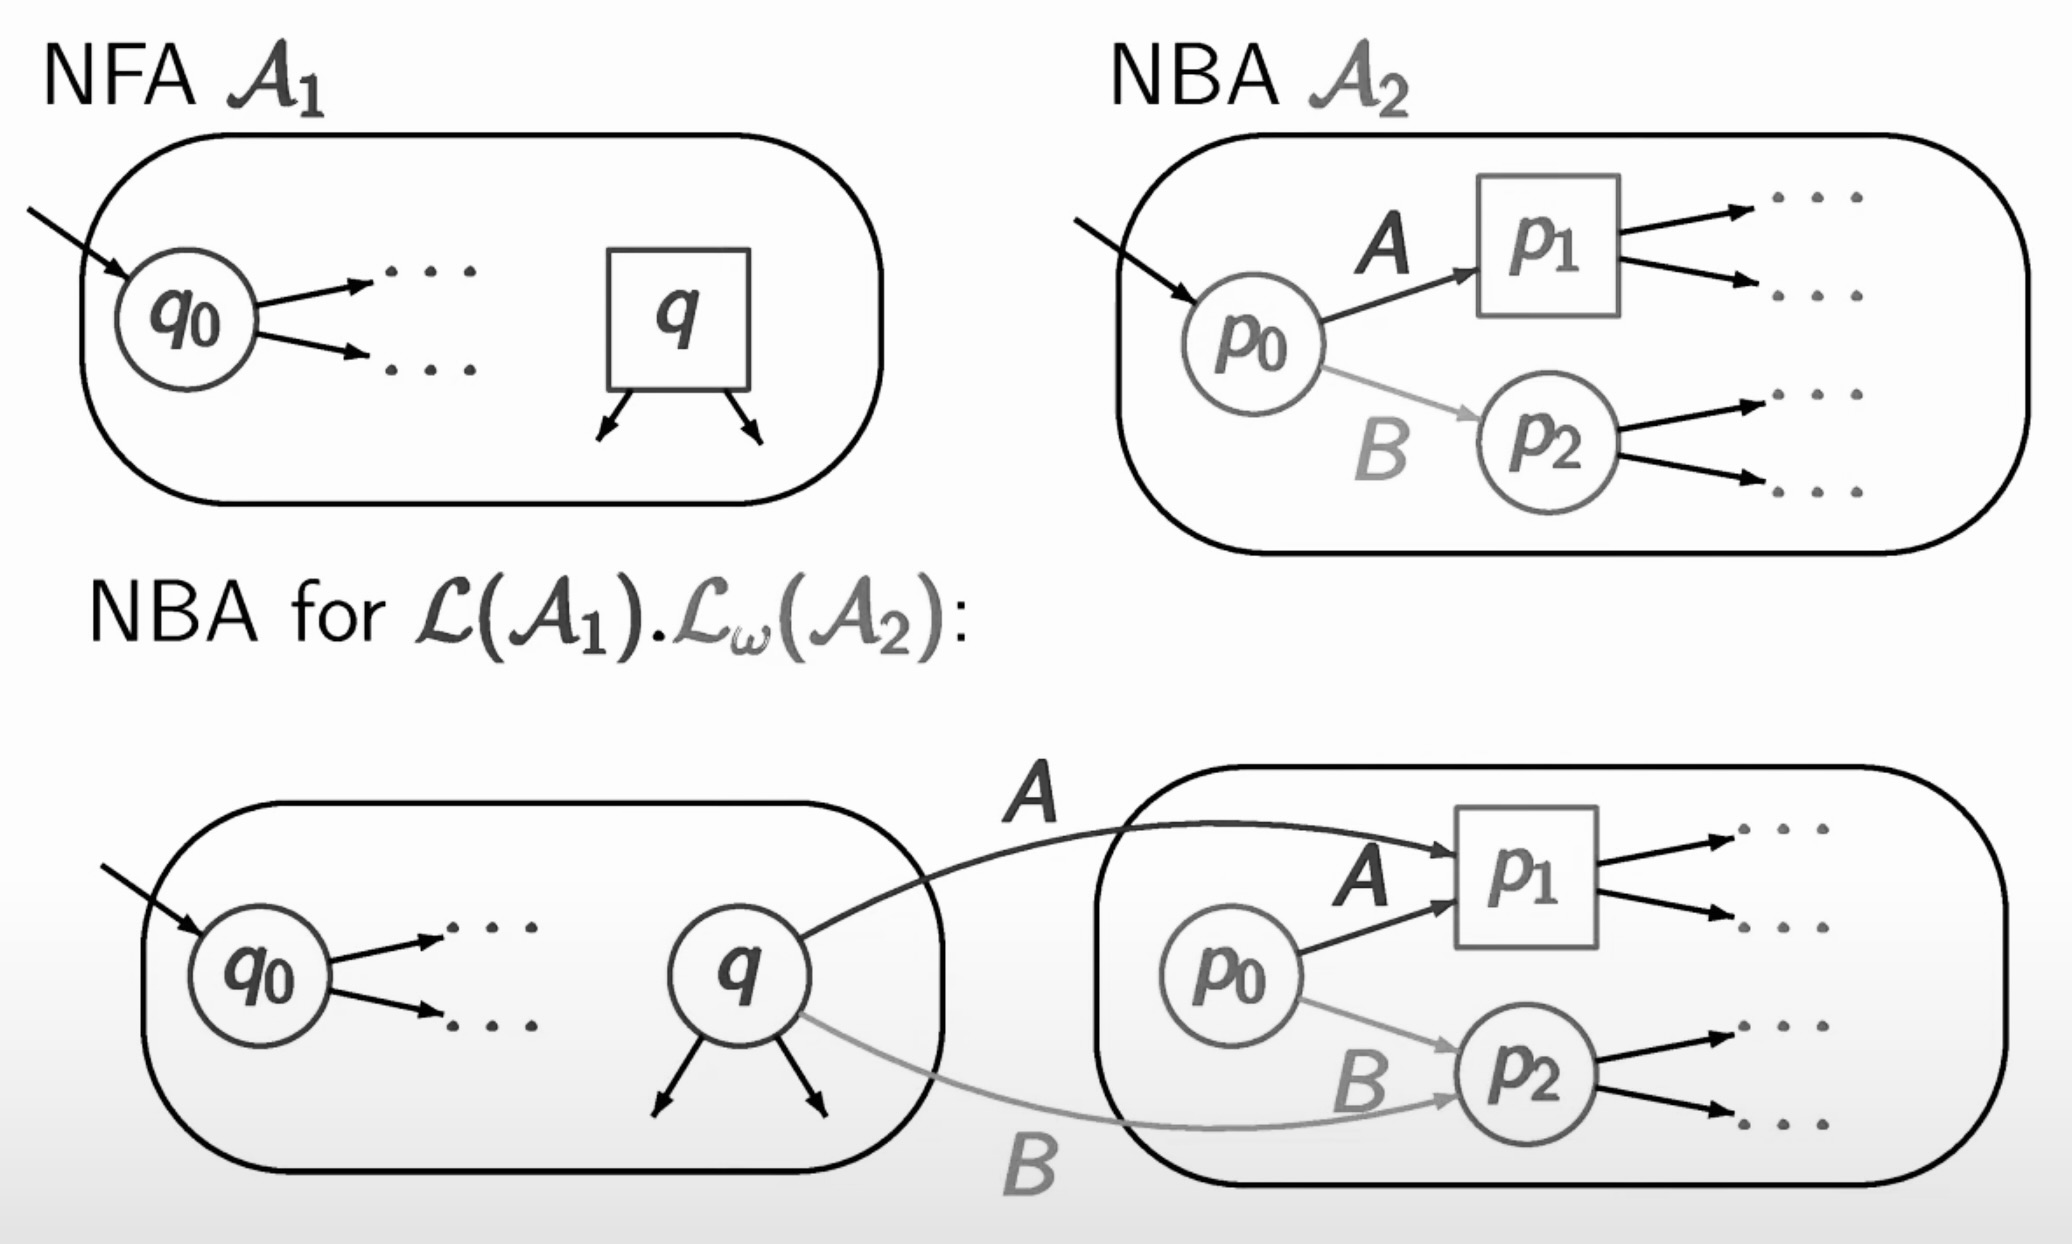
\includegraphics[width=1\textwidth]{photo2.jpeg}
      \end{figure}
    \end{frame}
    \begin{frame}{Concatenation of NFA and NBA}
      \begin{figure}
        \centering
        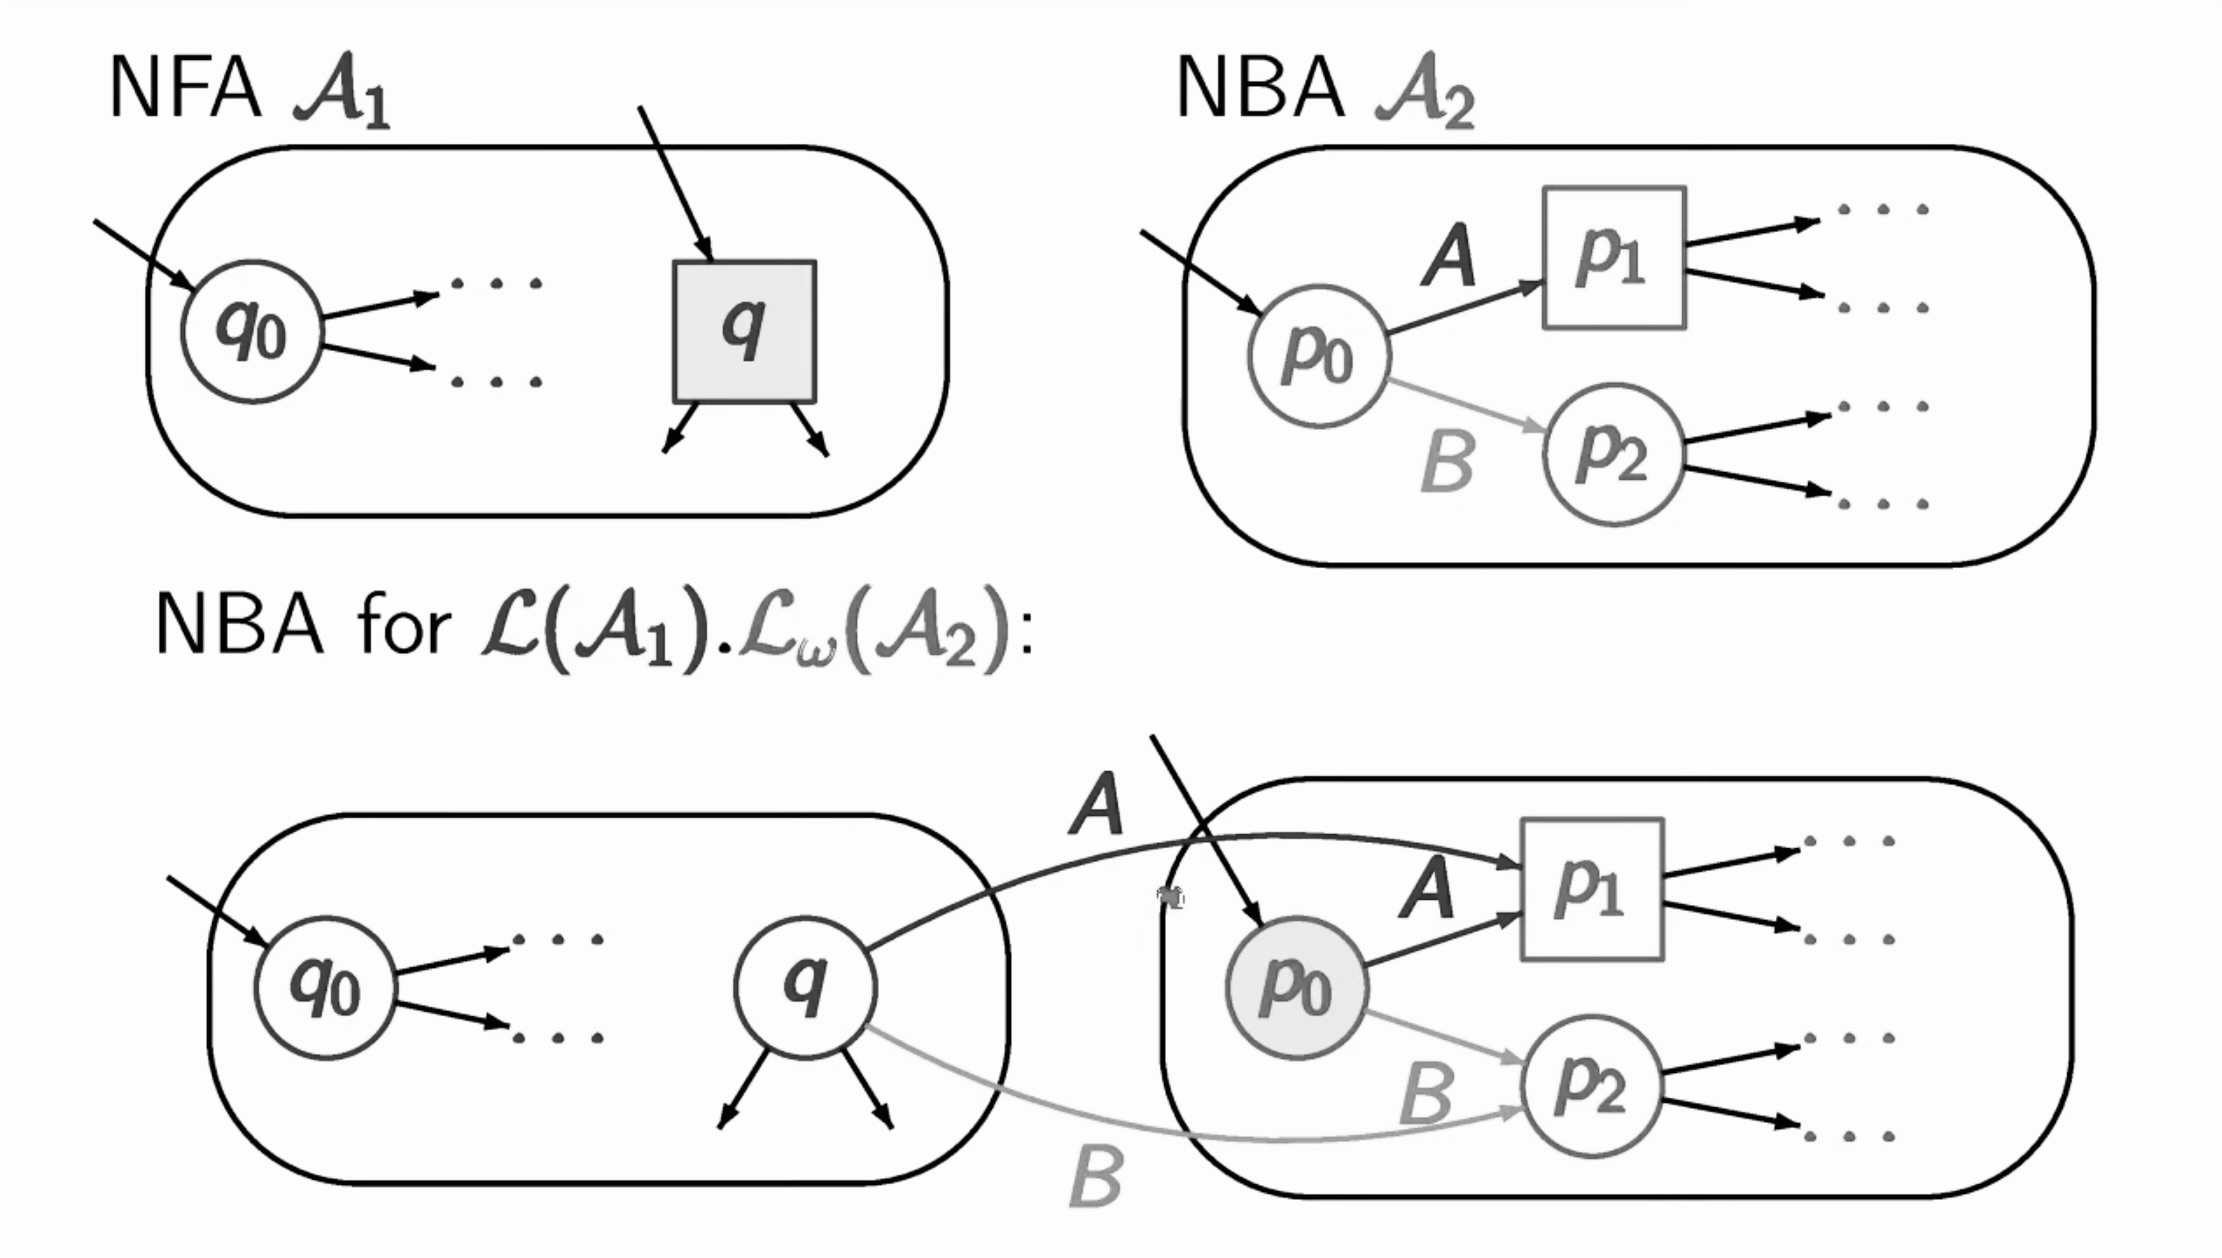
\includegraphics[width=1\textwidth]{photo3.jpeg}
      \end{figure}
    \end{frame}
    \begin{frame}{Construct NBA for NFA}
      \begin{columns}
        \column{0.5\textwidth}NFA $A$ for a language $\implies$ \\ $L \subseteq \Sigma^{+}$
        \begin{figure}
          \centering
          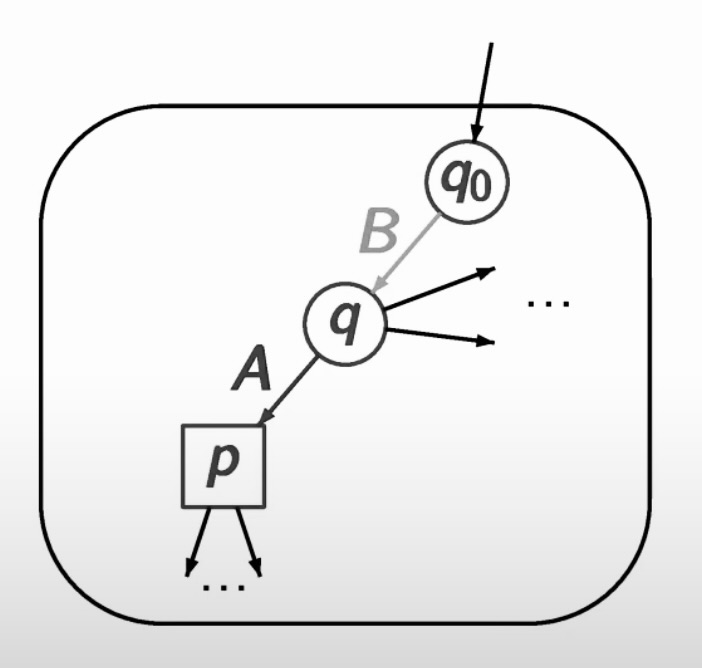
\includegraphics[width=0.8\textwidth]{photo5.jpeg}
        \end{figure}
        \column{0.5\textwidth} NFA  $\mathcal{B}$ for L such that all final states are terminal. 
        \begin{figure}
          \centering
          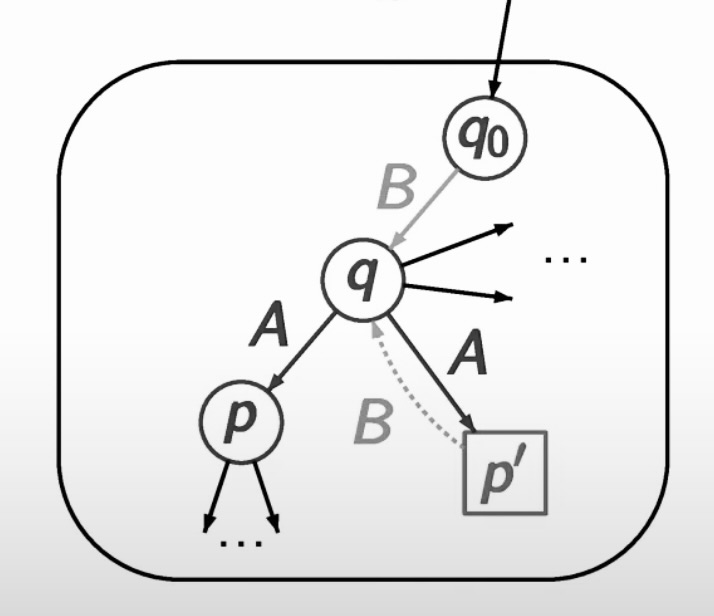
\includegraphics[width=0.8\textwidth]{photo6.jpeg}
        \end{figure}
      \end{columns}
      \[\mathcal{L}(A)^{\omega} = \mathcal{L}_{w}(\mathcal{B}^{\omega})\]
    \end{frame}
    \begin{frame}{Construct NBA for NFA}
      The final states (e.g. p) must be terminal states. If not make them.\\
      \alert{WHY ?}
      \onslide<2->{Because, if not, then there might be other possible paths introduced when we make the final state an "initial state" in the NBA.} 
    \end{frame}
    \begin{frame}{Example: Construct NBA for NFA}
      \begin{figure}
        \centering
        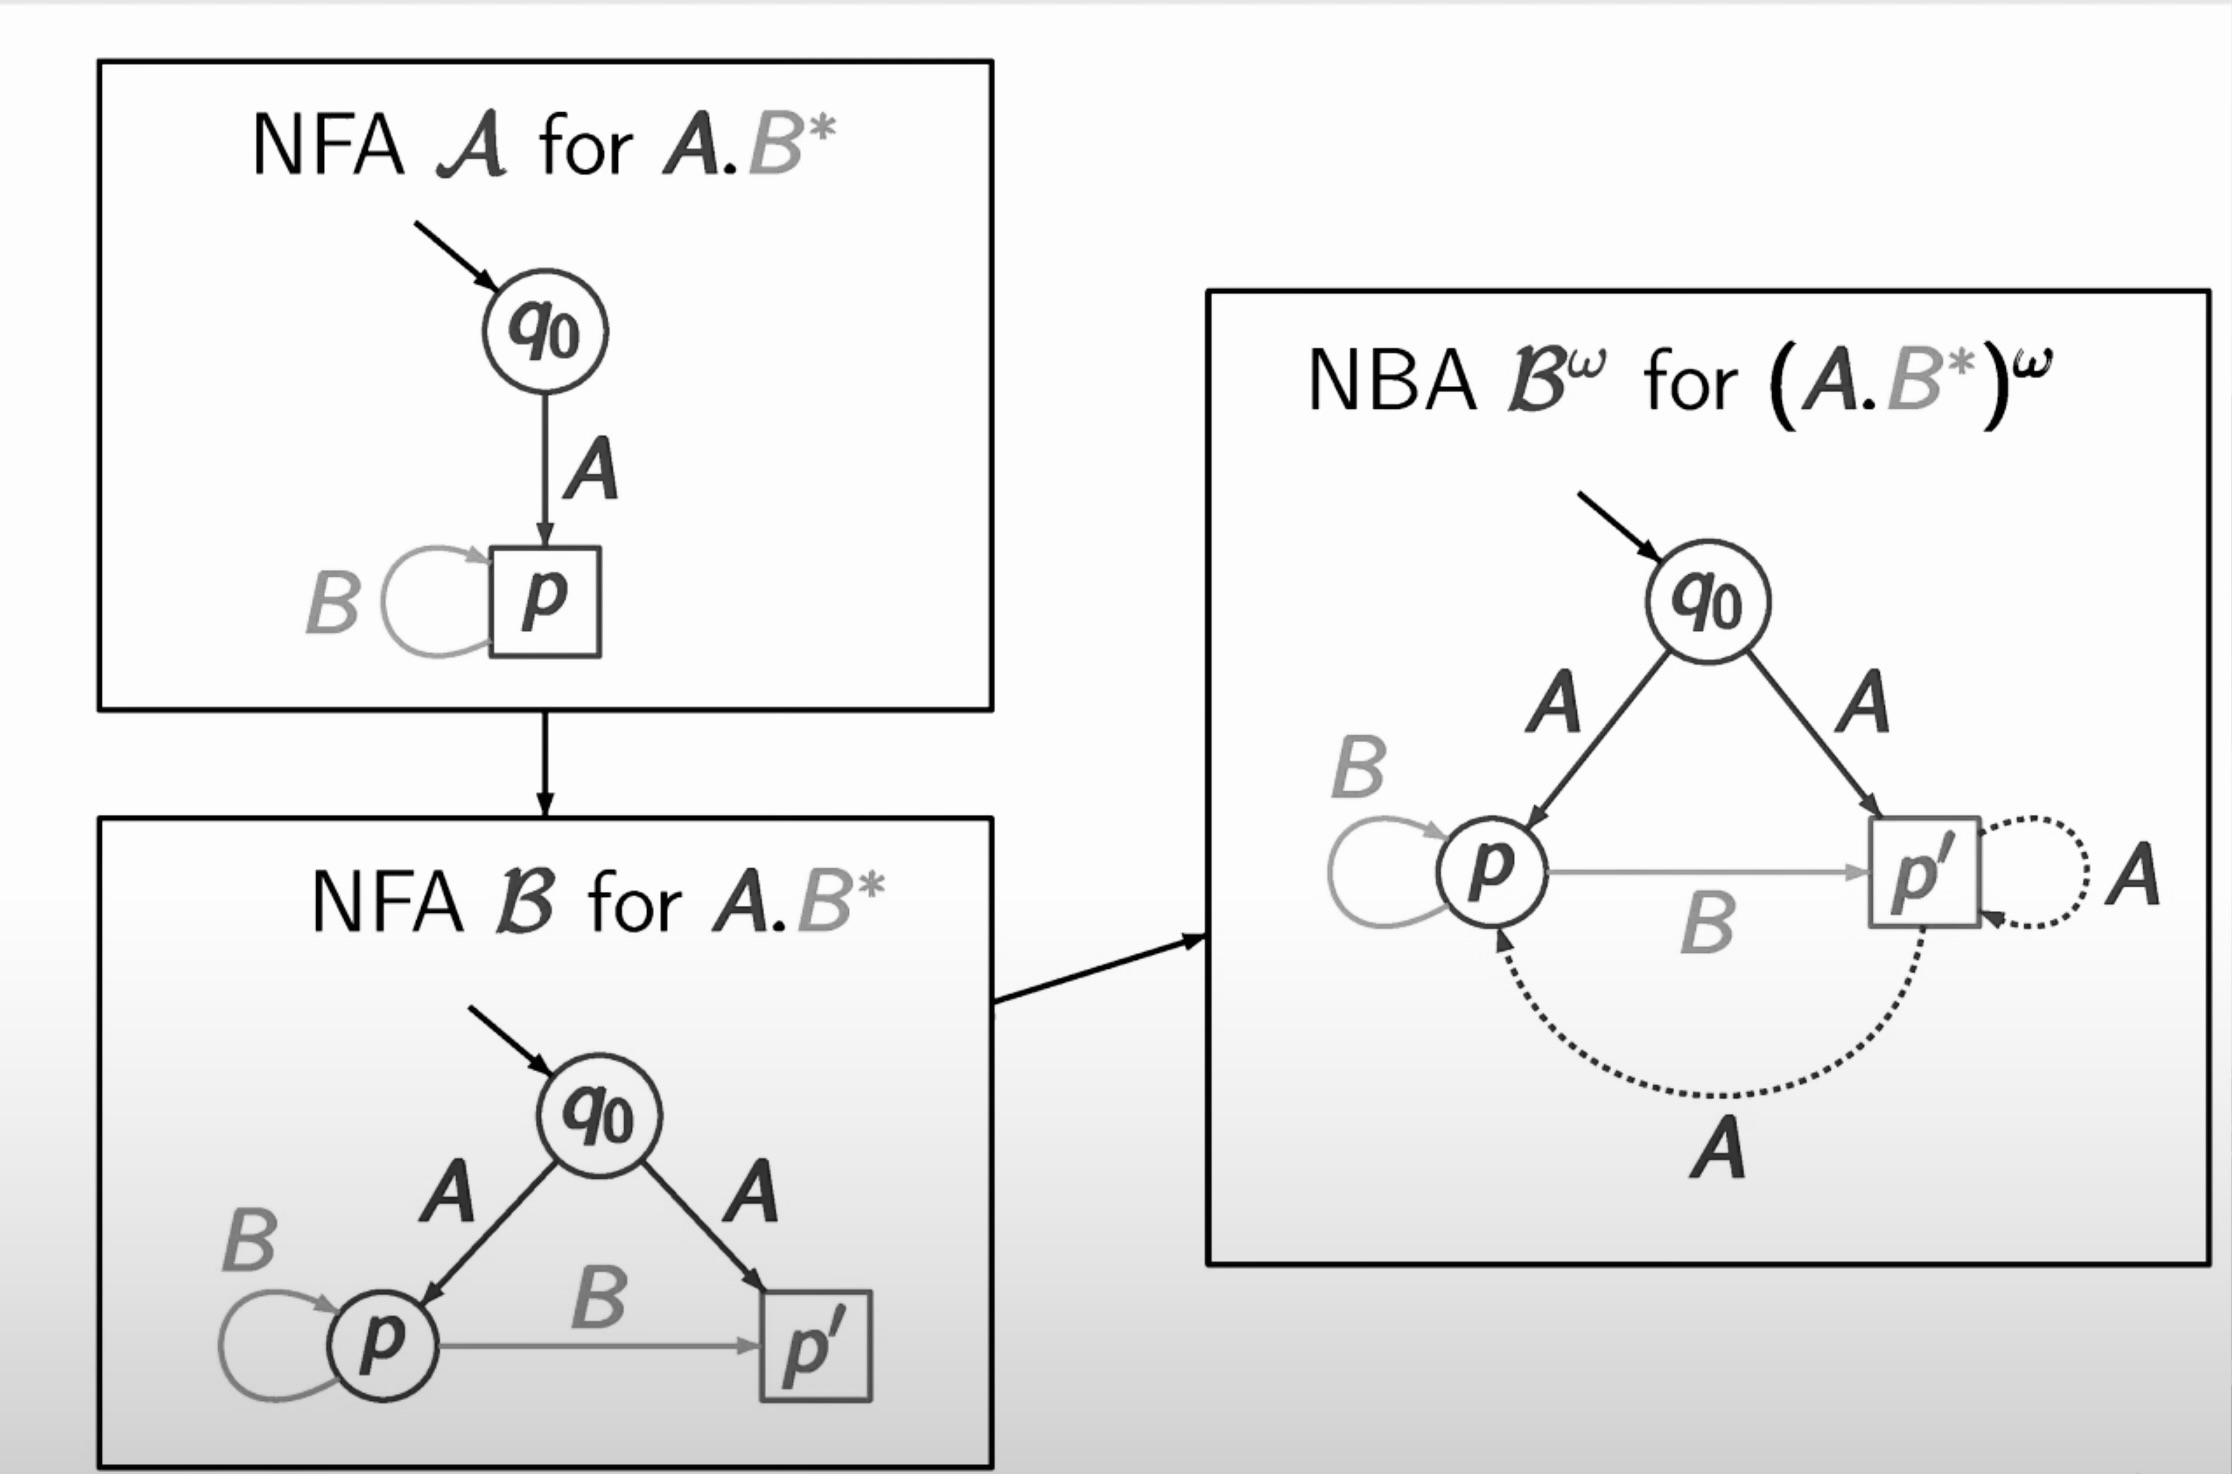
\includegraphics[width=1\textwidth]{photo4.jpeg}
      \end{figure}
    \end{frame}
    \section{Logic of Sequences and Büchi Automata}
    \begin{frame}{Logic of Sequences}

      Buchi’s original motivation for studying automata on infinite inputs was to solve a
  decision problem from logic. He discovered a deep and beautiful connection between
  $\omega$-regular languages and sets of models of formulas in certain logics.
    \end{frame}
    \begin{frame}{S1S}

      The logic that Buchi considered was the monadic second-order theory of one successor, abbreviated as S1S. This logic is interpreted over the set N0 of natural numbers.
      In general, second-order logic permits quantification over relations and functions,
      unlike first-order logic, which permits quantification over just individual elements.
      
      \begin{block}
      
        \begin{itemize}
          \item Second-order means that we allow quantifications over relations.
          \item Monadic means that quantifications is restricted to monadic relations, namely sets.
        \end{itemize}
      \end{block}
    \end{frame}
    \begin{frame}{S1S (contd.)}
      Fix a logical structure $(\omega, s, \in)$
      \begin{itemize}
        \item s is the successor function $x \rightarrow x + 1$
        \item $\in$ is the standard memebrship relation between elements and sets.
      \end{itemize}
      \begin{block}{Variables}
        \begin{itemize}
          \item First-order variables (x, y, z, etc.) range over natural numbers.
          \item Second-order variables (X, Y, Z, etc.) range over sets of natural numbers.
        \end{itemize}
      \end{block}
      \begin{block}{Terms}
        \begin{itemize}
          \item First-order variables are terms.
          \item If t is a term, then so is s(t)
        \end{itemize}
      \end{block}
    \end{frame}
    \begin{frame}{S1S (contd.)}
      \begin{block}{Formulas}
        \begin{itemize}
          \item Atomic formulas are of the form $t \in X$ where t is a term and X is a second-order variable.
          \item S1S formulas are built up from atomic formulas using standard boolean connectives, with $\forall$ and $\exists$ quantifications over first-order and second-order variables.
        \end{itemize}
      \end{block}
    \end{frame}
    \begin{frame}{Satisfiability and Buchi's Theorem}
      An S1S formula is said to be satisfiable if we can choose $M$ such that $M \vDash \phi$
      \begin{block}{Buchi's Theorem}
        Buchi showed how to associate an $\omega$-regular language $L_{(\phi)}$ with each S1S formula
$\phi$, such that every word in $L_{\phi}$ represents an interpretation for the free variables in
$\phi$ under which the formula $\phi$ evaluates to true. Moreover, every interpretation that
makes $\phi$ true is represented by some word in $L_{\phi}$. Thus, $\phi$ is satisfiable iff there
is some interpretation that makes it true iff $L_{\phi}$ is non-empty. 
      \end{block}
      \begin{example}
        Let $\phi$ be a invariant with invariant condition, $a \vee \neg b$. Then the $\omega$- regular language 
        associated with the invariant condition is $(\phi + \{a\} + \{a, b\})^{\omega}$ where $\phi $ is the empty set.
      \end{example}
    \end{frame}
    \begin{frame}{Motivation}
      \begin{itemize}
        \item<1-> Büchi automata's primary application is in formal verification of hardware and software systems.
        \item <2-> They are used to verify the correctness of systems that are infinite-state, such as communication protocols, distributed systems, and embedded systems.
        \item <3-> By infinite state, we mean the system runs indefinitely.
        \item <4-> Büchi automata are used to verify the correctness of such systems by checking if the system satisfies a given property.
        \item <5-> The property is usually specified as a formula in a temporal logic, such as LTL or CTL.
      \end{itemize}
    \end{frame}
      \begin{frame}{The end}
        \centering
        \only<1>{References:
        \begin{itemize}
          \item \url{https://www.youtube.com/watch?v=0Vnth-1X-OE&t=2290s&ab_channel=songsong}
          \item \url{https://www.cmi.ac.in/~madhavan/papers/pdf/iisc2011-buchi.pdf}
          \item \url{https://www.cs.ox.ac.uk/people/luke.ong/personal/talks/s1s.pdf}
          \item \url{https://medium.com/@sakshimahesh20/introduction-to-buchi-automata-c9e598935ab5}
        \end{itemize}}
        \only<2>{\Huge Thank You!}
      \end{frame}
\end{document}